\documentclass[twocolumn]{aastex62}

\newcommand{\vdag}{(v)^\dagger}
\newcommand\aastex{AAS\TeX}
\newcommand\latex{La\TeX}
\usepackage{amsmath}
\usepackage{physics}
\usepackage{hyperref}
\usepackage{natbib}
\usepackage[T1]{fontenc}
\usepackage[english]{babel}
\usepackage[utf8]{inputenc}

\begin{document}

\title{\Large Foreløpig ingen tittel.}

\author{Håkon Tansem}

\author{Nils-Ole Stutzer}

\author{Bernhard Nornes Lotsberg}

\begin{abstract}

\end{abstract}

\section{Introduction} \label{sec:intro}
An ever occuring problem in many fields of science is a binary system of
interacting elements taking two possible values. Binary problems can be found in
everything from political science, where one could model outcomes of a vote in a
two party system, to modeling phase transitions in solid states physics. In this
paper we will focus on the latter, where we will model a time evolving
two-dimensional Ising model of interacting spins by means of a Markov Chain
Monte Carlo (MCMC) algorithm in addition to a Metropolis algorithm. We will explore how
different grid sizes and temperatures make the lattice behave, and how the systems energy and magnetisation
developes in time, the final aim being to estimate the critical temperature of
the phase transition when the lattice looses its magnetisation. This is then
compared to the analytical value found by \cite{onsager:1944}. 

This paper will present needed theory and implementation of the theory in the Method
section \ref{sec:method}, the results will be presented in the Results section
\ref{sec:results} and be discussed in the Discussion section
\ref{sec:discussion}.

\section{Method} \label{sec:method}
\subsection{The Ising Model and Important Quantities from Statistical Menchanics} \label{subsec:ising_model}
The physical system considered by this paper will be a two-dimensional Ising
model, consisting of a grid of $N\times N$ magnetic spins. Each spin can have
the value $s = +1$ ($\uparrow$) or $s = -1$ ($\downarrow$), and they interact only with their nearest neighboors. An
example of such a lattice is 
\begin{align}
	\begin{smallmatrix}
		\uparrow & \downarrow & \cdots &\uparrow \\
		\uparrow & \uparrow & \cdots & \downarrow \\
		\vdots & \ddots & \ddots & \vdots \\
		\downarrow & \uparrow & \cdots & \uparrow.
	\end{smallmatrix}
\end{align}
The energy of the lattice is defined by 
\begin{align}
	E = -J\sum_l\sum_{\langle kl\rangle} s_k s_l,
	\label{eq:energy}
\end{align}
where $\langle kl\rangle$ denotes the sum over the nearest neighboors and the
spins take the values $s_i = \pm 1$ and $J$ has units energy. When counting the
energies we choose to use periodic boundaries, meaning that the nearest
neighboor of a spin $s_{i,N-1}$ at the edge of the lattice is the spin $s_{i,0}$
at the opposite edge of the lattice. This is done so as to simulate a lattice
that extends infinitly in space. Note that it is the interaction between two
neighbooring spins that contribute to the energy, thus each pair only needs to
be counted one time.
The magnetisation is defined similarly as 
\begin{align}
	M = \sum_i s_i,	
	\label{eq:magnetisation}
\end{align} 
simply being the sum of the systems spins. The probability density function (PDF) of the system having
a cetain energy state is given by the Boltzmann distribution 
\begin{align}
	P(E_i) = \frac{1}{Z}e^{-\beta E_i},
\end{align}

where $\beta = \frac{1}{k_B T}$ for the Boltzmann constant $k_B$ and the
temperature $T$. The partition function of the system discribing all statistical
properties of the system in equilibrium and is needed to normalize the Boltzmann
distribution is defines as the sum 
\begin{align}
	Z = \sum_{i = 1}^{2^{N^2}} e^{-\beta E_i},
\end{align}
over all possible microstates of the system. The mean energy and absolute magnetisation
of the system is then given as 
\begin{align}
	\langle E \rangle &= \sum_i E_i P(E_i) = \sum_i \frac{E_i}{Z}e^{-\beta E_i} = \pdv{\ln Z}{\beta}\\
	\langle |M| \rangle &= \sum_i |M_i| P(E_i) = \sum_i \frac{|M_i|}{Z}e^{-\beta E_i} 
\end{align}
and represent the most likely state of equilibrium of the system.
Another important quantity from
thermodynamics is the heat capacity measuring the change in temperature $T$ for
a given change in the systems heat. The heat capacity at constant volume is given as 
\begin{align}
	C_V &= \dv{\langle E \rangle}{T} = \frac{1}{k_B T^2}\left(\frac{1}{Z}\sum_i E_i^2 e^{-\beta E_i} - \langle E\rangle^2\right) \\
	& = \frac{1}{k_BT^2}\left(\langle E^2\rangle - \langle E\rangle^2\right) = \frac{\sigma^2_E}{k_B T^2},
\end{align}
thus being analogous to the variance in energy states. The sum again runs over
all microstates.
Finally, the magnetic susceptibility measuring how the systems magnetisation
responds to an external magnetic field, is defined as 
\begin{align}
	\chi &= \beta\left(\sum_i\frac{M_i^2}{Z}e^{-\beta E_i} - \langle |M_i|\rangle^2 \right)\\
	& = \frac{1}{k_BT}\left(\langle M^2\rangle - \langle |M|\rangle^2\right) = \frac{\sigma^2_{|M|}}{k_BT}.
\end{align} 
These thermodynamical quantities will later be usefull when estimating the
critical temperature of the phase transition when the system looses its net
magnetisation.
When later implementing these thermodynamical quantities numerically we will
use natural units where $k_B = 1$ and the energy is in units $J/k_B$, the
temperature will have dimensions energy $k_BT/J$. Also the magnetisation is in
this case a unitless quantity, and due to the energy and temperature scaling the
heat capacity and (HUSK ENHETER)

\subsection{Analytical Solutions to the $2\times2$ Lattice}\label{subsec:two_by_two_lattice}
Before discribing the algorithm modeling the time development of the lattice, we
show the analytical solutions to the mean energy and absolute magnetisation as
well as the heat capacity and the susceptibility, so as to later enable a
comperison of the numerical results to known analytically quantities. When
counting the energy and magnetisation of the $2\times2$ lattice as discribed in
the previous subsection we get the possible states of the system shown in Table
\ref{tab:possible_energy}. This lattice has in all $2^{N^2} = 2^4 = 16$ possible microstates. 

\begin{deluxetable}{cccc}
	%\tablewidth{0pt}
	\tablecaption{Table showing the possible energies $E_i$ and magnetisations $M_i$ of the $2\times2$ lattice and their corresponding number of spins up $N_\uparrow$ and their degenrecies $d_i$. \label{tab:possible_energy}}
	%\tablecomments{}
	\tablecolumns{4}
	\tablehead{$N_\uparrow$ & $d_i$ & $E_i$ $[J]$ & $M_i$}
	\startdata
	$4$  & $1$ & $-8$& $4$   \\
	$3$ & $4$  & $0 $& $2$\\
	$2$ & $4$  & $0 $& $0$\\
	$2$ & $2$  & $8 $& $0$\\
	$1$ & $4$ & $0 $& $-2$\\
	$1$ & $1$ & $-8$ &$-4$ 
	\enddata
\end{deluxetable}
Using the possible energy states in Table \ref{tab:possible_energy} we can write
the partition function of the system as 
\begin{align}
	Z &= \sum_i e^{\beta E_i} = e^{8J\beta} + 4 + 4 + 4 + 2e^{-8J\beta} + e^{8J\beta} \\
	&= 4\cosh(8J\beta) + 12.
\end{align}
Using this we get the expectation value for the energy to be  
\begin{align}
	\langle E\rangle  &= \frac{1}{Z}\sum_i E_i e^{-E_i\beta} \\
	&= \frac{1}{Z}\left(-8J + 2\cdot 8Je^{-8J\beta} - 8Je^{8J\beta}\right) \\
	&= -\frac{8J\sinh(8J\beta)}{\cosh(8J\beta) + 3}.
\end{align}
Similarly we find that the expectation value of the absolute magnetisation is
given by 
\begin{align}
	\langle |M| \rangle &= \frac{1}{Z}\sum_i |M_i|e^{-E_i\beta} \\
	&= \frac{1}{z}\left(4e^{8J\beta} + 4\cdot 2 + 4\cdot 2 4e^{8J\beta}\right) \\
	&= \frac{2e^{8J\beta} + 4}{\cosh(8J\beta) + 3}.
\end{align}
Next this leads to the heat capacity being 
\begin{align}
	C_V &= \dv{\langle E \rangle}{T} = -\frac{1}{k_BT^2}\dv{\langle E\rangle}{\beta} \\
	&= -\frac{1}{k_BT^2}\dv{\beta}\left(-\frac{8J\sinh(8J\beta)}{\cosh(8J\beta) + 3}\right) \\
	&= \frac{192(\cosh(8J\beta) + 1)}{k_B T^2(\cosh(8J\beta) + 3)^2},
\end{align}
and the susceptibility (when using the absolute magnetisation) is 
\begin{align}
	\chi_{|M|} &= \frac{1}{k_BT}\left(\langle M^2 \rangle - \langle |M|\rangle^2 \right) \\
	&= \frac{1}{k_BT}\left(\sum_i \frac{M_i^2}{Z}e^{-E_i\beta} - \langle |M|\rangle^2\right) \\
	&= \frac{1}{k_BT}\left(\frac{8e^{8J\beta} + 8}{\cosh(8J\beta) + 3} -\frac{(2e^{8J\beta} + 4)}{(\cosh(8J\beta) + 3)^2} \right).
\end{align}

These analytical quantities can now be compares to the numerical results.

\subsection{The Markov Chain Monte Carlo Algorithm}
Now that we have looked at how the lattice of interactign spins is set up, we
can begin discribing the algorithm used to simulate the evolution of the lattice
in time. The algorithm used to simulate the time evolution of the lattice is a
Markov Chain Monte Carlo algorithm. We will, however, only outline the algorithm
used here, which is derived in detail in Ch. 13 by \cite{jensen:2015}. 

The first step in the algorithm is to compute the initial energy and magnetisation of a
lattice of size $N\times N$, which can be ordered or disordered, depending on the
wanted simulation.
This is simply done by using (\ref{eq:energy}) and \ref{eq:magnetisation} as
discribed previously.

We simulate the time evolution by looping through a number of $M$ Monte Carlo
cycles. Then at each Monte Carlo cycle we sweep through the lattice $N\times N$
times and at each sweep we pick a random grid point $i, j$. We sweep over random
grid points $N\times N$ times to roughly ensure that the whole grid is covered.
Each sweep is in practice done by
simply drawing a random index from a uniform distribution $i,j\in[0, N-1]$,
using a Mersenne-Twister pseudo-random number generator. At the random grid
point we compute what energy the lattice would have if we were to flip the spin
around. Since each spin only has four different nearest neighboors contributiong
to
the energy we find that the change in energy for any suggested flip is among
five possible values $\Delta E \in {-8J, -4J, 0, 4J, 8J}$. Both the change in
energy $\Delta E$ and the change in magnetisation $\Delta M$ from a spin flip have analytical
expression;
\begin{align}
	\Delta E &= E_2 - E_1 = -J\sum_{\langle kl\rangle}s_k^2s_l^2 + J\sum_{\langle kl\rangle}s_k^1s_l^1 \\
	&= -J\sum_{\langle kl\rangle}s_k^2(s_l^2-s_l^1) = 2s_l\sum_{\langle k\rangle} s_k,
\end{align}
since the surrounding spins $s_k = s_k^1 = s_k^2$ are unchanged and the fliped
spin $s_l^2 = -s_l^1$. The magnetisation change is 
\begin{align}
	\Delta M = 2s_l^2,
\end{align}
since the difference in magnetisation at a spin flip is 2. 

The energy difference plays a key role when determaining if the suggested spin
flip should be accepted. The acceptance rule will be modelled by a Metropolis
algorithm and will be discribes in the next subsection. 

In case the spin is fliped we update the mean values $\langle E \rangle$ and
$\langle |M| \rangle$ and the variances $\sigma_E^2$ and $\sigma_{|M|}^2$, then
jumping to the next Monte Carlo cycle. If the flip is not accepted no changes to
the means and variances is made.

This is done for each Monte Carlo cycle. When letting the number of Monte Calro
cycles increas the system will than gradually converge towards the most likely
state $\langle E \rangle$, eventually oscillating around it. The computed sample
means and variances will than gradually approach the true means and variances.

One could alternatively to flipping each spin individually generate a new random
lattice and compute the total energy difference for each Monte Carlo to deterain whether
the new configuration should be accepted. However, this is extremely
inefficient, as it reequires many more FLOPs per Monte Carlo cycle than if each
spin is fliped individually.

\subsection{The Acceptance Rule - The Metropolis algorithm}
When modeling the acceptance rule we use the Metropolis algorithm. We will here
only outline the implementation of the Metropolis algorithm used following the
derivation done in Ch. 13 \cite{jensen:2015}. Since we don't know the transition
probability when suggesting a spin flip, we can model it by looking at the ratio
between the Boltzmann distribution of the state after and before the suggested
flip 
\begin{align}
	\frac{P(E_2)}{P(E_1)} = \frac{\frac{1}{Z}e^{-\beta E_2}}{\frac{1}{Z}e^{-\beta E_1}} = e^{-\beta\Delta E},
\end{align}
so as to eliminate the partition function, which becomes hard to calculate as
the grid increases since it contains a sum over $2^{N^2}$ microstates. This can
quickly result in overflow. The naive way to mode the transition would be to
only accept transitions into a lower energy state, i.e. where $\Delta E < 0$, as
a system generally tends towards the state of lowest energy. However, we don't want the
system to accept exlusively lower energies, as this is a major source of bias,
because the system than just quickly will freeze at the lowest energy state
possible. We therefore model the transition rule as 

\begin{align}
	r \leq e^{-\beta\Delta E},
\end{align}
where $r\in [0, 1]$ is a number drawn from a uniform PDF. Since $e^{-\beta\Delta
E}$ can be either greater or smaller than one, the transition rule can also make
the system transition to a less likely state once in a while. Therefore the
system will tend towards the equilibrium state, eventually oscillating arount
it, but never totally freeze.
Note that sice we know all the possible values of $\Delta E$ we can precalculate
the possible values of $e^{-\beta\Delta E}$, thus circumventing unnecessary
FLOPs.

\subsection{The Analysis}
Now that we have an algorithm computing the discribed thermodynamic quantites,
we can compare the output to the known analytical values for a $2\times 2$ grid
for say a temperature $k_BT/J = 1.0$.

The next step would be to choose a larger lattice, for instance $N = 20$, both
with an ordered and disordered initial spin configuration. Then we let the
system run through a large number of Monte Carlo cycles, representing a long
time, and computing the sample mean of energy and absolute magnetisation
\begin{align}
	\langle E\rangle &= \frac{1}{m}\sum_{i = 1}^m E_i\\
	\langle |M|\rangle &= \frac{1}{m}\sum_{i = 1}^m |M|_i,
\end{align} 
at each Monte Carlo cycle $m$. This cumulative mean we can use to find how much
time, i.e. how many Monte Carlo cycles, the system needs to reach a state close
to the most likely state where $\langle E \rangle$ and $\langle |M|\rangle$
start flattening out in general.

This is important since we only want to sample energies and magnetisation for
the thermodynamical quantites $C_V$ and $\chi$ later when looking at the phase
transitions. 
Also we plot the number of accepted flips as a function of the Monte Carlo
cycles to see how much the system changes states at any given time.

To further see if the lattice behaves as expected we can approximate the
Boltzmann distribution $P(E)$ for a given temperature $k_BT/J$ by making a
histogram of the energy states of the system. We would expect that for a low
temperatue like $k_BT / J = 1.0$ that $P(E)$ approaches a $\delta$-function at
small energies as
$\beta$ becomes large, and the exponential function $P(E)$ quickly dies out when
energies become larger. The lattice effectively freezes at the lowest possible
energy state. Therewhile for higher temperatures like $k_BT/J$ the PDF
will look more like a Gaussian distribution as the system has meany more
possible (symetric) energy states around the equilibrium that it can oscillate
around. 

The distributions are than compared to the sample variance given by the central
limit theorem \citep[p. 357]{jensen:2015} defined as 
\begin{align}
	\sigma^2 = \frac{\sigma^2_E}{m},
\end{align}
for the number of experiments (Monte Carlo cycles) $m$ and the energy variance
$\sigma_E^2 = \langle E^2\rangle - \langle E \rangle^2$. This will be an error
estimate of the statistical experiment as it measures the deviation between the
true mean and the sample mean. Also the spread in the histogram is compared to
the standard diviation $\sigma_E$.

Next, we want to study the phase transition where the lattice goes from having a
magnetisation to loosing its net magnetisation. We follow here the theory presented
by \cite{jensen:2019}. Near the critical temperature
$T_C$ for when the lattice undergoes the phase transition, the mean magnetisation is
given by 
\begin{align}
	\langle M(T) \rangle \sim (T-T_C)^\beta,
\end{align}
where $\beta = 1/8$ is the so-called critical exponent. The heat capacity and
the susceptibility follow a analogous relation as
\begin{align}
	C_V(T) &\sim |T_C - T|^\alpha \\
	\chi(T) &\sim |T_C - T|^\gamma,
\end{align}
where $\alpha = 0$ and $\gamma = 7.4$. When the lattice is heated to $T \gg T_C$
the correlation length $\xi$ of the lattice becomes of the order of the lattice size.
The correlation length is a measure of how far two correlated spins are
separated. As the temperatue $T$ appreaches the critical temperature $T_C$, the
correlation length increases as more and more of the lattice spins are correlated, exerting a divergent behaviour close to $T_C$ as 
\begin{align}
	\xi(T) = |T_C - T|^{-nu},
\end{align}
where we let $\nu = 1$. Since we study a second order phase transition the
correlation length will eventually span the whole system, corresponding to the
lattice size $N$ in our case since we are limited to a finite grid. Therefore since
$\xi\propto N$ we get that 
\begin{align}
	T_C(N) - T_C(N\to\infty) = aN^{-1/\nu},
	\label{eq:temp_crit}
\end{align}
where $a$ and $\nu$ are constants. Then the mean magnetisation becomes 
\begin{align}
	\langle M(T)\rangle \sim (T - T_C)^\beta \to N^{-\beta/\nu},
\end{align}
the heat capacity becomes 
\begin{align}
	C_V(T) \sim |T_C - T|^{-\alpha}\to N^{\alpha / \nu}
\end{align}
and the susceptibility is 
\begin{align}
	\chi(T)\sim |T_C - T|^{-\gamma} \to N^{\gamma/\nu},
\end{align}
where we have set $T_C(N) = T$ and $T_C(N\to\infty) = T_C$.
Thus if we plot the mean energy and magnetisation as well as the heat capacity
and susceptibility as a function of temperatres we can estimate the critical
temperature for an infinite grid $N\to \infty$. For this we use $N = 40, 60, 80$
and $100$, and a temperature range of $T\in[2.0, 2.5]$ with 50 temperature steps. We expect that the mean energy
and absolute magnetisation suddenly bend at $T = T_C(N)$, and that the heat
capacity and susceptibility peak at $T = T_C(N)$. When $N\to\infty$ this peak
will diverge. Using (\ref{eq:temp_crit}) for two grid sizes $N_1$ and $N_2$ we
can estimate the constant $a$ to be 
\begin{align}
	a = \frac{T_C(N_1) - T_C(N_2)}{N_1^{-1/\nu} - N_2^{-1/\nu}},
\end{align}
since we know that $T_C(N\to\infty)$ is the same for all grids. Knowing $a$ we
can use (\ref{eq:temp_crit}) to compute an estimate for $T_C(N\to\infty)$. This
estimate can be compared to the analytical value found by \cite{onsager:1944};
$k_BT/J = \frac{2}{\ln(1+\sqrt{2})}\approx 2.269$, for $\nu = 1$.
As looping over several temperatures using a desently large number of Monte
Carlo cycles is very time consuming, we parallelized the temperature loops using
MPI and used compiler flags. To check the speed-up we timed code using diffent
degrees of parallisation and compiler flags.

\section{Results} \label{sec:results}

\begin{figure*}
	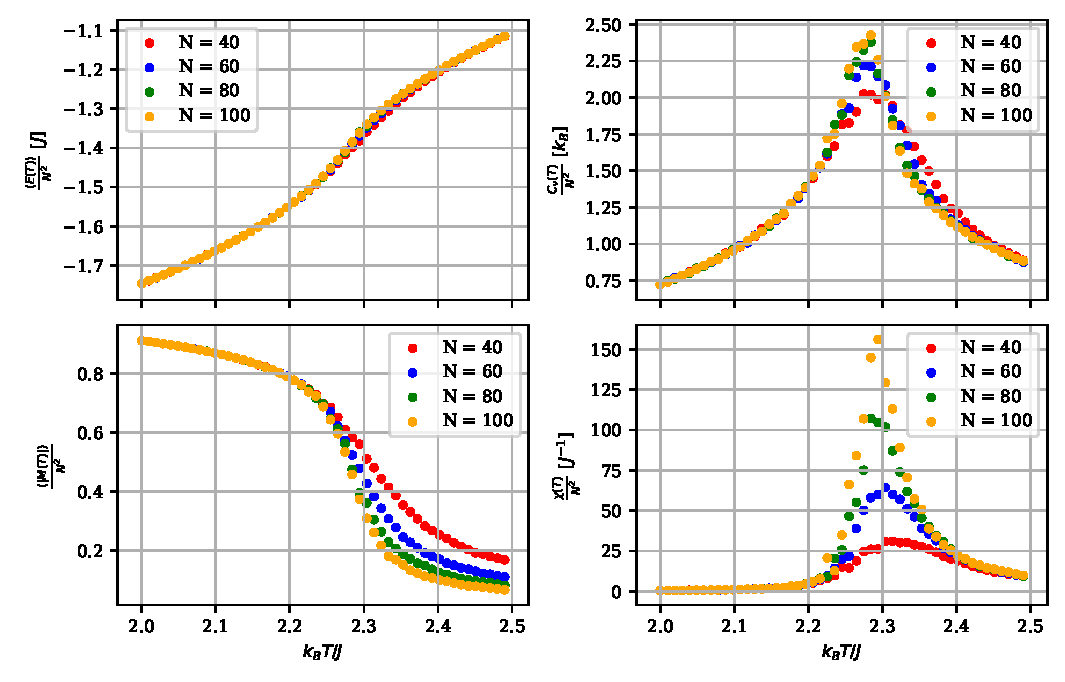
\includegraphics{{Figures/thermo_quants}.pdf}
	\caption{}
	\label{fig:thermo_quants}
\end{figure*}

\section{Discussion} \label{sec:discussion}

\section{Conclusion} \label{sec:conclusion}


\bibliography{ref}
\bibliographystyle{aasjournal}
\end{document}

% End of file `sample62.tex'.
